\documentclass{article}

\usepackage{epsfig}  
\usepackage{amsmath} 
\usepackage{amssymb} 
\usepackage{amsthm}  
\usepackage{listings} 
\usepackage{color}
%\usepackage{enumerate}
\usepackage{enumitem}
\usepackage{multirow}
\usepackage{lastpage}
\usepackage{geometry}
\usepackage{fancyhdr}
\usepackage[all]{xy}
\usepackage{wrapfig}
\usepackage{listings}
\usepackage{url}
\usepackage{tikz}
\usepackage{graphicx}
\usepackage{caption}
\usepackage{subcaption}
\usepackage[justification=centering]{caption}
\usetikzlibrary{arrows}
\lstset{language=C, tabsize=4, basicstyle=\ttfamily}

\definecolor{light}{gray}{.75} 
\newtheorem{theorem}{Theorem}

\newcommand\etal{\emph{et al.}}

\pagestyle{fancy}
\lhead{CSCE 990 - FALL 2014} 
\chead{\bfseries PROJECT PROPOSAL}
\rhead{Gerrard, Ore}
\lfoot{Gerrard, Ore}
\cfoot{\thepage\ of \pageref{LastPage}}
\rfoot{3 November 2014}
\renewcommand{\headrulewidth}{0.4pt}
\renewcommand{\footrulewidth}{0.4pt}

\hoffset 0pt
\voffset 0pt
\textwidth 15cm
\textheight 8.5in
\oddsidemargin 9pt
\marginparwidth 25pt
\setlength{\parindent}{0pt}
\setlength{\parskip}{.25cm}

%- - - - - - - - - - - - - - - - BEGIN DOCUMENT - - - - - - - - - - - - - - - - - - - 
\begin{document}


\section{Target Problem Description}



Model extraction seeks to help computer system developers understand complex systems by finding a simplified representation that retains useful high-level information.
This high-level information helps developers validate the system's behavior or to discover instructive counter-examples that violate implicit requirements. 
Robotic designers likewise work with highly complex systems and struggle to understand the complex interrelations between components as the robotic system moves though time and space.
Although model extraction tools like Synoptic~\cite{schneider2010synoptic} are useful for examining the relationships between temporal events, they have not, to our knowledge, been applied to spatial analysis for robotics. 
We seek to explore whether existing software model extraction tools can used to examine complex spatial events in robotic systems.

\section{Background}
A system's behavior is often recorded in system logs or execution traces, that provide some facts about the behavior of the system but are sometimes overwhelmingly massive and difficult to connect to high-level facts, even though these facts might reveal critical information about the behavior of the system.
%Tools that helps extract model from computer execution traces is Synoptic.
Synoptic takes system event logs as input and extracts high-level models based on calculating invariants and coarsening and refining an abstract model.
Synoptic and other tools usually work at an abstract level of system events, that happen in a particular order.
%The problem is to explore if model extraction techniques that are usually applied to temporal events (like network program execution traces) can be applied to spatial robotic data.
Given multiple runs of a robot completing some task, is it possible to use the traces of its sensor data to construct models of spatial events common to this task?

There are several challenges in this endeavor, including mapping existing robotic system trace data to \emph{events}, so that the spatial relationships of these events can be explored by extending previous model extraction techniques. 
This will include defining an event such as \emph{UP} as a change in the z-axis of 0.5 meters, for example, so that any fluctuations in the z-axis less than 0.5 meters will not be considered.  
The events will include basic spatial movements such as \emph{UP, DOWN, LEFT, RIGHT, FRONT, BACK} 
The next challange will be mapping sets of these events to higher-level spacial movements.  
For instance, a relatively equal number of \emph{UP}s followed by \emph{DOWN}s in an alternating pattern could be defined as \emph{BOUNCING}; similarly \emph{FRONT} alternating with \emph{BACK} could be \emph{PACING}.
We hope to characterize shapes of movements, so that a chain of \emph{FRONT,FRONT,RIGHT,BACK,BACK,LEFT} will be recognized as a \emph{RECTANGLE}.
It may also be useful to look at spatial constraints within event intervals.  
For example, we may want to know that within a certain state, the robot's motion is constrained to a consistently-sized sphere, or we may see that between two state changes, the robot is always below a certain altitude, etc.

\emph{Concrete example}
Consider the following position data coming from a trace of a robot's program execution:


xpos : 0.0519  ypos : 0.1742  zpos : 1.2231

xpos : 0.0831  ypos : 0.2014  zpos : 1.7469

xpos : 0.0427  ypos : 0.3003  zpos : 2.3333

xpos : 0.5843  ypos : 0.1967  zpos : 2.4091

xpos : 1.2082  ypos : 0.1861  zpos : 2.2984

xpos : 1.1549  ypos : 0.2989  zpos : 2.3003

xpos : 1.0227  ypos : 0.2117  zpos : 2.2811

xpos : 1.0519  ypos : 0.1647  zpos : 1.7210

xpos : 1.0813  ypos : 0.1539  zpos : 1.2093

xpos : 0.5003  ypos : 0.1702  zpos : 1.2151

xpos : 0.0001  ypos : 0.3099  zpos : 1.2177

xpos : 0.0103  ypos : 0.2774  zpos : 1.2031

The running program uses this data in a local context, so that a position value may trigger thrusters to activate in response to a gust of wind, but looking at the traces, you cannot easily derive what the robot actually \emph{did} in space.

%It is difficult to make any sense of this raw data.  
It is difficult to understand the relationships between high-level events by examining this low-level data.  
Because this kind of position data is often published in a periodic stream, the higher-level events are lost in the overwhelming quantity of lower-level data.
The \emph{xpos} value might change every millisecond, but if these values only fluctuate within a small range, you want to ignore these data points.  
Creating a set of events will make meaningful spatial movements easier to handle by only considering user-defined importance.  

\emph{Why does this matter?}  

A robot run may fail, perhaps due to a program crash or an uncompleted task.  
If the failure was not directly observed, if it is not directly linked to program calls which may be observed through dynamic invariant or modeling tools (Daikon, Synoptic), and if there are no helpful error messages, then you may want to examine its spatial behavior around failure states.
Given multiple traces of failed runs, you could see that the failure is always preceded by some spatial event, or only occurs within some constrained spatial region.
Comparing the ``success" and ``failure" spatial models against one another may give you insight to how the robot reacts to its environment which existing tools do not capture.
Analyzing spatial models across runs may also help improve the efficiency of robotic tasks.  
A model may reveal unnecessary pacing back and forth when the task at hand does not require this behavior; observing this may help the developer remove the superfluous motion.

\emph{Why are existing studies, techniques, or tools insufficient?}

There are currently no tools we are aware of that can extract models of general spatial events based on trace data. 
Synoptic can extract models based on temporal properties, and Daikon can extract invariants from traces, but these properties are often independent of the spatial models we hope to build.
Both Synoptic and Daikon build their models/invariants around method calls and object values, but in a reactive environment, the execution of code may only model a part of how the robot moves through space.
Additionally, these tools cannot meaningfully handle the large amounts of noise inherent to raw positional data.
Kuipers~\etal examined how robots can build a spatial map from trace data~\cite{kuipers1988robust}, but this is one map specific to a particular environment.
Similarly, Elfes~\cite{elfes2013occupancy} demonstrated a real-time spatial representation for robot perception, but this also addresses single runs in a particular environment and does not examine the relationships between spatial events at an abstract level.
Our tool will not try to build a precise map of the space in which it moves, but instead will look at general spatial events that occur across many runs of a task.

\section{Sketch of technique}

We start with robotic system traces from ROS, a published-subscriber architecture for connecting robotic components.  
These traces are called `bags' within the domain of ROS, and contain system messages published on certain data structures (called topics) in chronological order.
Specifically, we will examine trace data from a UAV system used to collect water samples during windy conditions.
Each file might contain 100,000 records, and we have 50-100 bags.

\emph{The ``how" details}

Starting with these bags, we plan to create functions that recognize certain sequences and values of message and record `events' to a new event log.
This event log captures important spatial events during the execution of an automated script, or plan, that lasts about five minutes.
One of the challenges will be creating the functions that recognize these events and determining the correct level of refinement for these events.

At a high level, the stages of model extraction will be:

\begin{itemize}
  \item For each bag file: BAG $\rightarrow$ BAG' $\rightarrow$ BAG'' 

  \item Process the entire collection of BAG'' files to return a spatial model.
\end{itemize}

% This still needs quite a bit of work/editing/thinking...

For each bag file, we will identify basic ``events" that will make up a new BAG' file.  
For this descriptive example, we will only consider the \emph{UP} event, but the technique is the same for the other primitive events.  
First the user will define a granularity of movement significance, such as 0.2 meters, so that any primitive movement which exceeds 0.2 meters will register as an event (or concatenation of events).
We will run checks on each publication of the position data, and if the z-axis position has increased by more than 0.2 meters, we will divide the increase by 0.2, take the floor of the result, call it x, and will write x instances of UP to the BAG' file.  
After we have a BAG' file that logs our primitive events, we will perform a linear scan on this file to check for each spatial property we are interested in.  
For instance, to check for any \emph{BOUNCING} intervals, we will scan the BAG' file for alternating consecutive \emph{UP}s and \emph{DOWN}s. 
These spacial events will be written to a BAG'' file.
The system we will be using publishes a global ``Subject Control State."
So to provide a rough grouping as we scan for each new spatial event, we will write the spatial events to the BAG'' file under the heading of their respective states.
This grouping will hopefully become less coarse throughout the course of implementation.
From the collection of BAG'' files, we will note behaviors which occur more than a predefined number of times as ``common" behaviors to each state for that given task.

\emph{Tool applied to example}

% This will demonstrate our example being parsed to the events "FRONT,FRONT,LEFT,LEFT,LEFT,BACK,BACK,RIGHT,RIGHT,RIGHT" which will then be translated to a "RECTANGLE" event
% How contrived! How trivial! Ah well...
% Because the example doesn't deal with multiple trace bag files, we will explain how a rough model might be extracted from multiple "RECTANGLE" events occuring in state 8...

Applying our tool to the example trace data, assume we set the meaningful primitive events to occur with every change in 0.5 meters. 
As the first BAG' file of primitive events is being created, each row is compared against its immediate successor by examining the difference between the corresponding coordinates.
Examining the first two rows of the example, for the "xpos" change we get $0.0831-0.0519=0.0312$, which is below the threshold of 0.5 meters, so no event in the x-axis will be recorded.  
Similarly, with "ypos", the difference is $0.2014-0.1742=0.0272$, which is also below 0.5, and no event in the y-axis will be recorded.
With "zpos", the difference is $1.7469-1.2231=0.5238$, which is above 0.5 meters, and because it is a positive increase in the z-axis, an event of \emph{UP} will be written to the BAG' file.

Processing all the rows in this way gives a bag file with the series of events: 

\emph{UP,UP,RIGHT,RIGHT,DOWN,DOWN,LEFT,LEFT}

As we process the BAG' file, this series of events will be recognized as a \emph{RECTANGLE} spatial event, which will be written to the BAG'' file.  
Our small example does not deal with multiple bag files, but the idea is that all these bag files will be parsed into separate BAG'' files, and if the above \emph{RECTANGLE} event occured each time in "State 8", then the model will state that in "State 8," the event \emph{RECTANGLE} is probable to occur.

\emph{Techniques/tools/frameworks to be used}

We will write the tool using a scripting language, either Ruby or Python.
We use the idea of confidence thresholds from Daikon to determine when some spatial property is considered "regular" as opposed to "random" across runs. 
For the model extraction component of our tool, we will use segment and interval trees to determine when events occur within states and/or across multiple states.
The spatial events will be based on "templates" which are defined by the occurrence and order of specified primitive events.
We may find it useful to define our primitives in the language of spatial logic found in Peuquet~\etal and spatial constraints found in Bindiganavale~\etal. 

\emph{Description of Solution}
% will add other metrics/clean this up

The precision will be as fine or as coarse as the user defines.
If the user defines events as only registering every 2 meters, a model may be quickly built, but the results may be unhelpful.
If the user defines events as registering every 0.00001 meters, the model will follow the trace data exactly, and the excess information will take a long time to process and will return too many spatial events.
The completeness will also depend on user-defined confidence thresholds.
If some event always occurs or occurs frequently, this property will be captured; if it seldom occurs, it will not be captured.  

\emph{Small Study}

Using a UAV in the NIMBUS lab, we will fly it in certain patterns over multiple runs and see if our tool can derive these spatial properties from the bags.
We will first start with our contrived example of moving in a rectangular motion.  
If this is feasible, we will include multiple events in a single run, such as bouncing followed by rectangular motion.
We will also include periods of erratic motion to see if our tool incorrectly constructs models where none would seem to exist.
If time allows, we may want to consider the partial and total orders of spatial relations, such as "above," "below," "in front of," and "behind" with respect to planes in space.

%\begin{figure}[b]
    %\centering
    %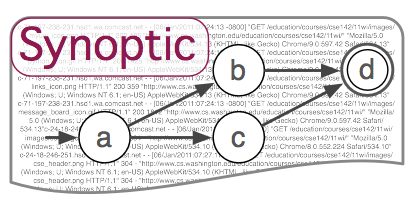
\includegraphics[width=0.4\textwidth]{./figures/TBD.jpg}
    %\caption{Awesome Image}
    %\label{fig:awesome_image}
%\end{figure}


\section{Expected Outcome} 

\emph{Connections with analyses studied in class}

As we hope to infer spatial models from trace data over multiple runs, our proposed tool shares many similarities with Daikon, which infers program invariants from (possibly) multiple runs given some input.
Like Daikon, we hope to work backwards from the trace data; because of this, like Daikon, the quality/correctness of the models we extract will be closely tied to the quality/robustness of the input data set.
We have also taken the idea of confidence thresholds from Daikon, to determine when a spatial event occurs with regularity, and when it just happened to occur a limited number of times.
Unlike Daikon, we are not looking at invariants, so our models can be much more lax; if a spatial property is missing from some traces, but is present in most, we will still include this property in the model.
The publisher/subscriber architecture that captures events during a robot's task is similar to instrumenting your code to output desired variable values (Valgrind, Daikon).
However, raw sensor data is different than instrumented code because these sensors will output periodically, regardless of whether values have changed, and this creates a lot of data noise which must be filtered.
The way we will extract models from multiple BAG'' files (containing spatial events) may employ methods of time-series (state-series in our case) analysis and multivariate analysis which are used in Jenkins.  
We hope to use the spatial models to identify behavior around areas where runtime failures occur, though this will not be an automatic recovery, as in Carzaniga~\etal.

\emph{Advances in state of practice/art}

\bibliographystyle{IEEEtran}
\bibliography{IEEEabrv,refs.bib}

\end{document}
